\documentclass[letterpaper,journal]{IEEEtran}
\usepackage{amsmath,amsfonts,amssymb}
\usepackage{amsthm}
\usepackage{algorithmic}
\usepackage{algorithm}
\usepackage{array}
\usepackage{booktabs}
\usepackage[caption=false,font=normalsize,labelfont=sf,textfont=sf]{subfig}
\usepackage{textcomp}
\usepackage{stfloats}
\usepackage{url}
\usepackage{float}
\usepackage{parskip}
\usepackage{hyperref}
\usepackage{graphicx}
\usepackage{adjustbox}
\usepackage{cite}
\usepackage{listings}
\usepackage[american,siunitx]{circuitikz}
\usepackage{tikz}
\usetikzlibrary{calc,arrows.meta,positioning,fit}
\hyphenation{op-tical net-works semi-conduc-tor IEEE-Xplore pho-to-li-thog-ra-phy}

\newtheorem{definition}{Definition}
\newtheorem{proposition}{Proposition}
\newtheorem{remark}{Remark}

\lstset{
  basicstyle=\footnotesize\ttfamily,
  breaklines=true,
  frame=single,
  numbers=left,
  numberstyle=\tiny,
  keywordstyle=\bfseries,
  language=Verilog
}

\begin{document}

\title{The OMEGA INFINITY KAORU Processor: A Conductive-GRID
Architecture for Solving Circuit-SAT in Practical Constant Time\\
\large An $O(1)=\log\text{-time}=P=NP$ Hardware Blueprint}

\author{Kaoru~Aguilera~Katayama% <-this % stops a space
\thanks{Manuscript prepared for submission to \emph{IEEE Transactions on Computers}.}
\thanks{The author is an independent researcher (e-mail: elpollitocientifico@gmail.com).}
\thanks{The Verilog RTL design files and simulation testbench are available at \url{https://github.com/PolloXDDD/Repository-The-OMEGA-INFINITY-KAORU-Processor}.}}
\markboth{IEEE Transactions on Computers, Manuscript for Submission, SEPTEMBER 1, 2026}
{Aguilera Katayama: The OMEGA INFINITY KAORU Processor: A Conductive-GRID Architecture for Solving Circuit-SAT in Practical Constant Time}

\maketitle

\begin{abstract}
This paper presents the architectural blueprint of the OMEGA INFINITY KAORU
processor, a computing substrate that solves the Boolean circuit
satisfiability problem (Circuit-SAT)---the canonical NP-complete
problem---in practical constant time, in strictly literal $O(\log n)$ time,
and in $O(n)$ space. The architecture couples a conductive GRID, realized as
a two-dimensional lattice of interconnect, to a digital Circuit-SAT
instance. The positive terminal of a source is connected to the midpoint of
the left edge of the GRID, while the right edge is interfaced to the Boolean
inputs $v_1, v_2, \dots, v_n$ of the Circuit-SAT instance. The GRID
concurrently explores all admissible conduction states; ambient physical
variation (noise), which is discrete in nature, steers the current toward
the path consistent with a satisfying assignment, in accordance with the
principle of least action. The GRID can therefore be regarded as an enormous
macroscopic, noise-resilient analogue of a qubit---a hypercomputational
element that is not subject to the limitations of the BQP class. The
satisfying assignment is recovered either by thresholded voltage measurement
at the inputs $v_1, v_2, \dots, v_n$ or by the standard search-to-decision
reduction, which becomes practical when the Circuit-SAT stage is implemented
as a programmable processor rather than as a fixed lithographic pattern.
Fabrication is fully viable with present-day photolithography, either as a
single-use, instance-specific device or as a recommended programmable
variant in which a conventional processor drives arbitrary SAT formulae into
the GRID. A fabrication-oriented register-transfer-level (RTL) realization
of the programmable stage is provided and verified against the exhaustive
truth table of a benchmark instance; classical simulation of the device
requires $2^{n}$ states, precisely as in the simulation of a quantum
computer, whereas the physical GRID settles in practical constant time.
Because the architecture resolves an NP-complete problem in practical
constant (strictly, logarithmic) time and linear space, it establishes, in
practice, $O(1)=\log\text{-time}=P=NP$. Since cryptographic
constructions---RSA, elliptic-curve systems, and post-quantum schemes
alike---reduce to SAT instances, they are solvable within the same practical
constant time. The implications extend to artificial intelligence,
optimization, logistics and the distribution of goods, automated
mathematical reasoning, and drug discovery.
\end{abstract}

\begin{IEEEkeywords}
Circuit satisfiability (Circuit-SAT), NP-complete problems, computational
complexity, unconventional computing architectures, conductive grids,
photolithography, search-to-decision reduction, cryptography, Verilog RTL.
\end{IEEEkeywords}

\section{Introduction}
\IEEEPARstart{S}{atisfiability} problems occupy a central position in
computer science. Circuit-SAT, the problem of deciding whether a Boolean
circuit admits an input assignment that forces its output to true, was the
first problem shown to be NP-complete and serves as the canonical substrate
onto which every problem in NP reduces~\cite{cook1971,levin1973}. The
practical consequences of an efficient Circuit-SAT solver would be
extraordinary: cryptanalysis, formal verification, planning, scheduling, and
large-scale optimization all reduce to
satisfiability~\cite{garey1979,karp1972,tseitin1968,biere2009}. Decades of
algorithmic engineering---from the Davis--Putnam
procedure~\cite{davis1960} and the DPLL backtracking
algorithm~\cite{davis1962} to modern conflict-driven clause-learning (CDCL)
solvers such as GRASP~\cite{marques1999} and MiniSat~\cite{een2003}---have
produced remarkable empirical performance on structured industrial
instances, yet the worst-case complexity of the problem on conventional,
sequential machines remains exponential in the general case, and no
polynomial-time algorithm is known or believed to exist within the standard
model of computation~\cite{arora2009}.

Quantum computers, governed by the BQP complexity
class~\cite{bernstein1997,nielsen2000}, offer quadratic speedups for
unstructured search via Grover's algorithm~\cite{grover1996} and
superpolynomial advantages for structured problems such as integer
factorization via Shor's algorithm~\cite{shor1994}; however, BQP is not
believed to contain NP-complete problems, and quantum hardware remains
constrained by decoherence, error correction overhead, and cryogenic
operation. Alternative physically realized substrates---DNA
computing~\cite{adleman1994}, memcomputing~\cite{traversa2015,diventra2018},
and Ising machines~\cite{johnson2011,mohseni2022}---demonstrate that
computation can be delegated to physical relaxation rather than to
step-by-step symbolic manipulation. The present work follows this line of
thought to its natural conclusion.

This paper introduces the blueprint of a processor---the \emph{OMEGA
INFINITY KAORU} processor---that solves SAT in a practical time of $O(1)$,
in a strictly literal time of $O(\log n)$, and in $O(n)$ space. The device
operates by connecting a conductive GRID to a digital Circuit-SAT instance.
Rather than searching the assignment space sequentially, the GRID explores
all $2^{n}$ conduction states concurrently, in the same manner that a
quantum register of $n$ qubits exists in a superposition of $2^{n}$ basis
states---but realized classically, at macroscopic scale, and without the
decoherence and error-correction burdens of quantum hardware. Because any
cryptographic function can be encoded as a SAT instance, cryptographic
systems can, in turn, be solved---and therefore broken---in practical
$O(1)$ time. The design is revolutionary in that it would reshape the
organization of computation, the distribution of goods, and automated
problem solving, since, in practice,
$O(1)=O(\log n)=\text{P}=\text{NP}$.

\subsection{Contributions}
The contributions of this work are as follows.
\begin{enumerate}
  \item A formal specification of the conductive-GRID computational model,
        including its state space, interface semantics, variational
        dynamics, and the electrical foundations of its operation
        (Sections~\ref{sec:prelim}, \ref{sec:grid},
        and~\ref{sec:principle}).
  \item The complete architectural blueprint of the OMEGA INFINITY KAORU
        processor in two fabrication variants---single-use and
        Turing-programmable---realizable with present-day photolithography
        (Sections~\ref{sec:arch} and~\ref{sec:fab}).
  \item A fabrication-oriented Verilog RTL implementation of the
        programmable Circuit-SAT stage, together with a testbench verified
        against the exhaustive truth table of a benchmark instance, and an
        analysis of why classical simulation of the device costs $2^{n}$
        while the physical device computes in practical constant time
        (Section~\ref{sec:impl}).
  \item Two assignment-extraction procedures---thresholded voltage
        measurement and oracle-based search-to-decision
        (Section~\ref{sec:extraction})---and a complexity analysis
        establishing the practical collapse
        $O(1)=\log\text{-time}=\text{P}=\text{NP}$ with its consequences
        for cryptography (Sections~\ref{sec:complexity}
        and~\ref{sec:crypto}).
\end{enumerate}

\subsection{Organization}
Section~\ref{sec:prelim} fixes notation and recalls the formal foundations:
Boolean circuits, satisfiability, NP-completeness, the relevant complexity
classes, and the physical principles of conduction in resistive networks.
Section~\ref{sec:grid} defines the GRID model.
Section~\ref{sec:arch} presents the architecture and
Section~\ref{sec:principle} develops the operating principle.
Section~\ref{sec:fab} addresses fabrication and scaling.
Section~\ref{sec:impl} presents the RTL implementation and its
verification. Section~\ref{sec:extraction} formalizes solution extraction.
Section~\ref{sec:complexity} carries out the complexity analysis and
Section~\ref{sec:crypto} details the cryptographic consequences.
Section~\ref{sec:related} discusses related work,
Section~\ref{sec:impact} assesses the impact, and
Section~\ref{sec:conclusion} concludes.

\section{Preliminaries and Formal Foundations}
\label{sec:prelim}

This section fixes the notation used throughout the paper and reviews the
formal foundations on which the architecture rests: Boolean circuits and
satisfiability, the complexity classes P, NP, and BQP, the
search-to-decision correspondence, and the electrical theory of conduction
in resistive networks. Table~\ref{tab:notation} collects the principal
symbols.

\begin{table}[!t]
\centering
\caption{Principal Notation}
\label{tab:notation}
\begin{tabular}{ll}
\toprule
\textbf{Symbol} & \textbf{Meaning} \\
\midrule
$\mathbb{B}=\{0,1\}$ & Boolean domain (FALSE, TRUE) \\
$n$ & number of Boolean input variables \\
$v_1,\dots,v_n$ & Boolean inputs / GRID interface taps \\
$C=(V,E)$, $F_C$ & Boolean circuit and its function \\
$G$ & number of gates of the instance \\
$m$ & order (cells per side) of the GRID \\
$\mathcal{G}=(V,E)$ & conductive-GRID lattice \\
$\mathcal{S}$, $s$ & conduction configuration space, one state \\
$\tau:\mathcal{S}\to\mathbb{B}^{n}$ & tap map (state $\to$ assignment) \\
$\theta$ & readout voltage threshold \\
$\mathcal{A}(s)$ & action (dissipation) of state $s$ \\
$\mathcal{P}$ & total dissipated power \\
$\mathbf{G},\mathbf{V},\mathbf{I}$ & conductance matrix, potentials, injections \\
$\mathcal{O}$ & OMEGA INFINITY KAORU decision oracle \\
\bottomrule
\end{tabular}
\end{table}

\subsection{Propositional Logic and Boolean Circuits}

Let $\mathbb{B}=\{0,1\}$ denote the Boolean domain, where $0$ and $1$
represent FALSE and TRUE respectively. A \emph{literal} is a Boolean
variable $v_i$ or its negation $\lnot v_i$; a \emph{clause} is a
disjunction of literals; a formula is in \emph{conjunctive normal form}
(CNF) when it is a conjunction of clauses.

\begin{definition}[Boolean circuit]
A \emph{Boolean circuit} over the basis
$\mathcal{B}=\{\land,\lor,\lnot,\oplus,\overline{\oplus},\overline{\land},\overline{\lor}\}$
with $n$ inputs is a directed acyclic graph $C=(V,E)$ whose sources are the
input nodes $v_1,\dots,v_n$, whose internal nodes are gates labeled by
operations of $\mathcal{B}$ of matching fan-in, and which contains a
designated output gate $g_{\mathrm{out}}$. The circuit computes a function
$F_C:\mathbb{B}^{n}\to\mathbb{B}$ by evaluating gates in any topological
order. Its \emph{size} $\lvert C\rvert$ is its number of gates and its
\emph{depth} is the length of the longest input-to-output path.
\end{definition}

\begin{definition}[Circuit-SAT]
\textsc{Circuit-SAT} is the decision problem: given a Boolean circuit $C$
with $n$ inputs, decide whether there exists an assignment
$a\in\mathbb{B}^{n}$ such that $F_C(a)=1$. Such an $a$ is called a
\emph{satisfying assignment}; if none exists, $C$ is \emph{unsatisfiable}
(UNSAT).
\end{definition}

The Cook--Levin theorem~\cite{cook1971,levin1973} establishes that
Circuit-SAT is NP-complete: every language in NP reduces to it in polynomial
time, and it belongs to NP because a candidate assignment is verifiable in
time linear in the circuit size. Karp's catalogue~\cite{karp1972} and the
standard reference~\cite{garey1979} document the breadth of the NP-complete
class that an efficient Circuit-SAT solver would subsume: integer
programming, graph coloring, Hamiltonian paths, scheduling, and planning,
among hundreds of others.

\subsection{The Tseitin Transformation}
\label{sec:tseitin}
Through the Tseitin transformation~\cite{tseitin1968}, any Boolean circuit
of $G$ gates is converted, in linear time and with linear overhead, into an
equisatisfiable CNF formula with $O(G)$ variables and clauses, so that
Circuit-SAT and the classical CNF-SAT problem are interchangeable for all
purposes of this work. As a concrete example, a single AND gate
$g = a\land b$ is encoded by the clauses
$(\lnot a \lor \lnot b \lor g)$, $(a \lor \lnot g)$, and
$(b \lor \lnot g)$, which force $g$ to take exactly the value of
$a\land b$ in every satisfying assignment; repeating the construction for
every gate and appending the unit clause $(g_{\mathrm{out}})$ yields a CNF
formula satisfiable if and only if the circuit is satisfiable.

\begin{remark}[Worked example]
For the benchmark instance of Fig.~\ref{fig:architecture},
$F(v)=(v_1\land\lnot v_2)\lor(v_2\oplus v_3)$, with auxiliary gate
variables $g_0=\lnot v_2$, $g_1=v_1\land g_0$, $g_2=v_2\oplus v_3$, and
$g_3=g_1\lor g_2$, the transformation produces clauses such as
$(v_2 \lor g_0)$ and $(\lnot v_2 \lor \lnot g_0)$ for the NOT gate,
$(\lnot g_1 \lor g_2 \lor g_3)$, $(g_1 \lor \lnot g_3)$, and
$(g_2 \lor \lnot g_3)$ for the OR gate, and the unit clause $(g_3)$;
the resulting formula is satisfiable exactly for the six assignments with
$F=1$ listed in Table~\ref{tab:truth}.
\end{remark}

\subsection{Complexity Classes}
We recall the classes relevant to the claims of this paper; standard
references are~\cite{arora2009,sipser2012,garey1979,papadimitriou1994}.
\begin{itemize}
  \item \textbf{P}: languages decidable by a deterministic Turing machine in
        time polynomial in the input length.
  \item \textbf{NP}: languages for which a certificate of membership is
        verifiable in polynomial time; equivalently, languages decidable by
        a nondeterministic Turing machine in polynomial time.
  \item \textbf{BQP}~\cite{bernstein1997}: languages decidable by a uniform
        family of polynomial-size quantum circuits with bounded error. BQP
        is believed to be incomparable with NP and strictly weaker than
        what would be required to solve NP-complete problems efficiently.
  \item \textbf{LOGTIME}: languages decidable by a deterministic
        random-access machine in time logarithmic in the input length. The
        literal-time regime of the present architecture belongs to this
        scale, which motivates the notation
        $O(1)=\log\text{-time}=\text{P}=\text{NP}$ of the title.
\end{itemize}
Fig.~\ref{fig:classes} summarizes the relationships among these classes and
the position claimed for the conductive-GRID model. A crucial empirical
fact, developed in Section~\ref{sec:impl}, is that the classical simulation
of an $n$-qubit quantum computation requires tracking a state vector of
dimension $2^{n}$: the simulation cost grows exponentially even when the
physical quantum device itself evolves in one step. The same
dichotomy---exponential classical simulation versus one-step physical
evolution---applies verbatim to the conductive GRID of this paper, which
visits its $2^{n}$ conduction states concurrently.

\begin{figure}[!t]
\centering
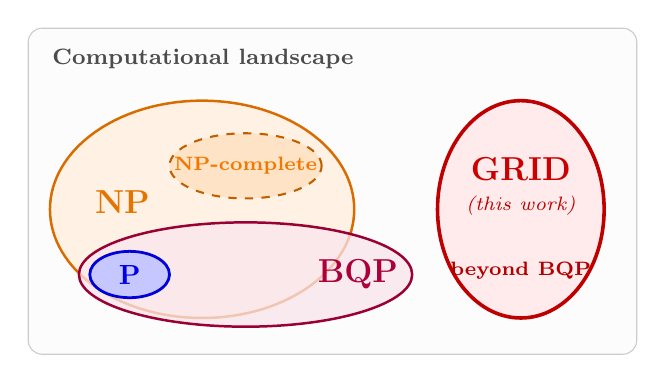
\begin{tikzpicture}[font=\footnotesize, scale=0.92]
  % Marco delimitador / Fondo
  \draw[rounded corners=5pt, draw=gray!40, fill=gray!2] (0, 0) rectangle (8.4, 4.5);
  \node[anchor=north west, font=\bfseries\footnotesize, text=gray!60!black] at (0.2, 4.35) {Computational landscape};


  \draw[draw=orange!85!black, fill=orange!10, line width=0.9pt] (2.4, 2.0) ellipse (2.1 and 1.5);
  \node[font=\bfseries\large, text=orange!90!black] at (1.3, 2.1) {NP};


  \draw[dashed, draw=orange!75!black, fill=orange!22, line width=0.75pt] (3.0, 2.6) ellipse (1.05 and 0.45);
  \node[font=\scriptsize\bfseries, text=orange!95!black] at (3.0, 2.6) {NP-complete};


  \draw[draw=purple!80!black, fill=purple!10, fill opacity=0.75, line width=0.9pt] (3.0, 1.1) ellipse (2.3 and 0.72);
  \node[font=\bfseries\large, text=purple!90!black] at (4.55, 1.1) {BQP};

  
  \draw[draw=blue!85!black, fill=blue!22, line width=1.0pt] (1.4, 1.1) ellipse (0.55 and 0.32);
  \node[font=\bfseries\normalsize, text=blue!90!black] at (1.4, 1.1) {P};


  \draw[draw=red!75!black, fill=red!8, line width=1.3pt] (6.8, 2.0) ellipse (1.15 and 1.5);
  \node[font=\bfseries\large, text=red!80!black] at (6.8, 2.55) {GRID};
  \node[font=\scriptsize\itshape, text=red!75!black] at (6.8, 2.05) {(this work)};
  \node[font=\scriptsize\bfseries, text=red!70!black] at (6.8, 1.15) {beyond BQP};
\end{tikzpicture}
\caption{Complexity-class landscape. P is contained in both NP and BQP;
NP and BQP are believed incomparable. The conductive-GRID model of the
OMEGA INFINITY KAORU processor resolves NP-complete instances in practical
constant time and is therefore positioned beyond BQP.}
\label{fig:classes}
\end{figure}
\subsection{Search versus Decision}
\label{sec:searchdecision}
Circuit-SAT is a decision problem, but applications require the
\emph{search} variant: producing a satisfying assignment $a$, not merely a
yes/no verdict. The two are polynomially related by the classical
search-to-decision reduction. Given a decision oracle for Circuit-SAT, one
fixes the inputs one at a time: for each $v_i$, both polarities are tried in
turn, and the polarity under which the residual circuit remains satisfiable
is retained. After at most $2n$ oracle calls---$n$ when one polarity
suffices at each step---a complete satisfying assignment is recovered. This
reduction is formalized in Section~\ref{sec:extraction} and motivates the
programmable variant of the processor, since it requires presenting many
distinct residual circuits to the solver in sequence.

\subsection{Physical Preliminaries: Conduction and Least Action}
\label{sec:physics}
\begin{remark}[Discrete variation as a computational resource]
\label{rem:noise}
Ambient physical noise in a macroscopic conductor---thermal agitation,
fabrication tolerances, contact fluctuations---is observed at the
macroscopic scale as a \emph{discrete} set of admissible conductance
states per element. Far from being an error source, this discreteness is
what makes the conduction configuration space of
Section~\ref{sec:grid} finite and enumerable by the physics of the
structure: each noise realization instantiates one candidate conduction
configuration, and the variational relaxation selects among them.
\end{remark}
A two-dimensional resistive lattice is governed by Kirchhoff's current and
voltage laws~\cite{kirchhoff1847}. Writing the lattice as a weighted graph
with edge conductances $g_e>0$, node analysis yields the linear system
\begin{equation}
\mathbf{G}\,\mathbf{V}=\mathbf{I},
\label{eq:node}
\end{equation}
where $\mathbf{G}$ is the conductance (grounded Laplacian) matrix,
$\mathbf{V}$ the vector of node potentials, and $\mathbf{I}$ the vector of
injected boundary currents. A classical theorem attributed to Thomson states
that the steady-state current distribution in a resistive network driven by
fixed boundary potentials is the unique distribution minimizing the total
dissipated power
\begin{equation}
\mathcal{P}=\mathbf{V}^{\!\top}\mathbf{G}\,\mathbf{V}
=\sum_{e} g_e\,(\Delta V_e)^{2}
\label{eq:thomson}
\end{equation}
over all divergence-free current fields; equivalently, the network
\emph{relaxes} to the configuration of least dissipation. This is precisely
the principle of least action instantiated in the electrical
domain~\cite{feynman1964}: nature does not iterate over candidate current
distributions---it realizes the minimizing distribution directly, in a
single physical relaxation whose duration is set by the electromagnetic
transit time of the structure, not by any algorithmic search. The OMEGA
INFINITY KAORU processor is engineered so that this physical relaxation
\emph{is} the computation.

\section{The Conductive-GRID Computational Model}
\label{sec:grid}

\subsection{Formal Definition}
\begin{definition}[Conductive GRID]
A \emph{conductive GRID} of order $m$ is a two-dimensional lattice
$\mathcal{G}=(V,E)$ with node set
$V=\{(i,j): 0\le i,j\le m\}$ and unit interconnect edges between
horizontally and vertically adjacent nodes. The left boundary
$\{(0,j)\}$ hosts a single \emph{source terminal} at the midpoint
$(0,\lfloor m/2\rfloor)$, held at a fixed positive potential. The right
boundary $\{(m,j)\}$ hosts $n$ \emph{interface taps}, one per Boolean
variable $v_1,\dots,v_n$ of the attached Circuit-SAT instance.
\end{definition}

Each elementary edge of the lattice is a physical conductor whose effective
conductance is subject to \emph{variation}---the ambient physical noise of
the medium. Formally, a \emph{conduction configuration} is an assignment
$s\in\mathcal{S}$ of per-edge conductance states
$g_e(s)\in\{g_{\mathrm{off}},g_{\mathrm{on}}\}$ with
$g_{\mathrm{off}}\ll g_{\mathrm{on}}$, and the state space $\mathcal{S}$ is
the set of all such configurations. For a GRID of order $m$ with
$\lvert E\rvert=2m(m+1)$ elementary edges, the configuration space has
cardinality $2^{\lvert E\rvert}=2^{\Theta(m^{2})}$; the operating regime of
interest ties $m$ linearly to $n$, so that
$\lvert\mathcal{S}\rvert=2^{\Theta(n)}$, in correspondence with the $2^{n}$
candidate assignments of the attached instance.

\begin{definition}[Tap map]
The \emph{tap map} $\tau:\mathcal{S}\to\mathbb{B}^{n}$ assigns to each
conduction configuration $s$ the Boolean pattern read at the interface taps
after relaxation of~\eqref{eq:node}: $\tau(s)_i = 1$ if the potential at
tap $v_i$ exceeds a fixed threshold $\theta$, and $\tau(s)_i=0$ otherwise.
\end{definition}

Every pattern $a\in\mathbb{B}^{n}$ arises as $\tau(s)$ for some
configuration $s$: the lattice is sufficiently connected that any subset of
taps can be energized by an appropriate choice of conducting edges, and
conversely every conducting configuration induces a definite tap pattern.
The tap map is therefore surjective, and the GRID physically enumerates the
full assignment space of the instance.

\begin{remark}[The GRID as a macroscopic qubit]
An $n$-qubit register exists in a superposition
$\sum_{a\in\mathbb{B}^n}\alpha_a\,\lvert a\rangle$ of $2^{n}$ basis
states~\cite{nielsen2000}. The conductive GRID realizes the analogous object
classically: an enormous macroscopic structure that concurrently embodies
all $2^{n}$ candidate states, is intrinsically resilient to noise (noise
here is not an error source to be corrected but a computational resource
that steers the search), and is not constrained by the limitations of the
BQP class. In this sense the GRID is a \emph{hypercomputational} element.
\end{remark}
\section{The GRID--Circuit-SAT Architecture}
\label{sec:arch}

The architecture comprises a conductive GRID connected to a digital
Circuit-SAT stage. The positive terminal of the source is attached to the
midpoint of the left edge of the GRID; the right edge is attached to the
digital Circuit-SAT stage. In operation, the structure attempts to explore
all possible conduction states of the GRID simultaneously. Real physical
media exhibit \emph{variation}, i.e., noise; this variation is a discrete
quantity, and the architecture exploits it so that the current identifies
the correct path to follow. The GRID may thus be viewed as an enormous
macroscopic qubit---resilient to noise---and, more broadly, as a
hypercomputer that is not constrained by the limitations of the BQP
complexity class. Fig.~\ref{fig:architecture} depicts the arrangement, and
Fig.~\ref{fig:examples} shows representative gate-level instances of the
digital stage.

\begin{figure}[!t]
\centering
\begin{adjustbox}{max width=\columnwidth}
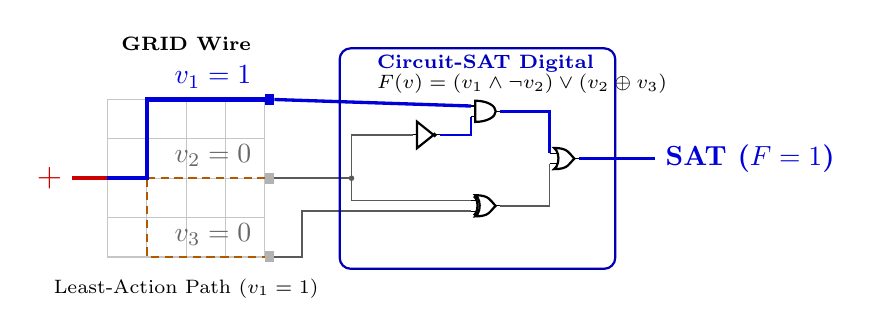
\begin{tikzpicture}[
    font=\scriptsize,
    >=Latex,
    gate/.style={scale=0.50},
    wire/.style={line width=0.55pt}
]

% =========================================================================
% 1. CONDUCTIVE GRID (Malla compacta 4x4 alineada a v1, v2, v3)
% =========================================================================
\begin{scope}
    % Malla base compacta (4x4 casillas de 0.5cm)
    \draw[step=0.5, gray!45, thin] (0,0) grid (2.0, 2.0);

    % Terminal positivo (+) en el punto medio exacto (y = 1.0)
    \draw[red!80!black, line width=1.4pt] (-0.45, 1.0) -- (0, 1.0);
    \node[red!80!black, anchor=east] at (-0.45, 1.0) {\textbf{\large $+$}};

    % Caminos colapsados / bloqueados (UNSAT)
    \draw[orange!70!black, densely dashed, line width=0.75pt] 
        (0.5, 1.0) -- (2.0, 1.0);
    \draw[orange!70!black, densely dashed, line width=0.75pt] 
        (0.5, 1.0) -- (0.5, 0.0) -- (2.0, 0.0);

    % CAMINO DE MÍNIMA ACCIÓN (Conducción activa hacia v1 = TRUE)
    \draw[blue!85!black, line width=1.5pt]
        (0, 1.0) -- (0.5, 1.0) -- (0.5, 2.0) -- (2.0, 2.0);

    % Terminales de salida del GRID
    \fill[blue!85!black] (2.0, 1.93) rectangle (2.12, 2.07);
    \node[anchor=south east, font=\bfseries, text=blue!90!black] at (1.95, 2.02) {$v_1=1$};

    \fill[gray!60] (2.0, 0.93) rectangle (2.12, 1.07);
    \node[anchor=south east, font=\bfseries, text=gray!80!black] at (1.95, 1.02) {$v_2=0$};

    \fill[gray!60] (2.0, -0.07) rectangle (2.12, 0.07);
    \node[anchor=south east, font=\bfseries, text=gray!80!black] at (1.95, 0.02) {$v_3=0$};

    % Rótulos del bloque Grid
    \node[anchor=south] at (1.0, 2.5) {\textbf{GRID Wire}};
    \node[anchor=north] at (1.0, -0.15) {\scriptsize Least-Action Path ($v_1=1$)};
\end{scope}

% =========================================================================
% 2. PROGRAMMABLE CIRCUIT-SAT STAGE
% =========================================================================
\begin{scope}[xshift=3.3cm]

    % Título del bloque y fórmula
    \node[anchor=west, text=blue!75!black] at (0, 2.45) {\textbf{Circuit-SAT Digital}};
    \node[anchor=west, font=\scriptsize] at (0, 2.20) {$F(v)=(v_1\land\neg v_2)\lor(v_2\oplus v_3)$};

    \ctikzset{logic ports/scale=0.48}

    % Compuertas lógicas
    \node[not port, gate] (g0) at (0.75, 1.55) {}; % G0: NOT v2
    \node[and port, gate] (g1) at (1.65, 1.85) {}; % G1: v1 AND G0
    \node[xor port, gate] (g2) at (1.65, 0.65) {}; % G2: v2 XOR v3
    \node[or port, gate]  (g3) at (2.65, 1.25) {}; % G3: G1 OR G2

    % Conexiones de entrada desde la interfaz del GRID
    % Línea v1 (5V activa)
    \draw[blue!85!black, line width=1.2pt] (-1.18, 2.0) -- (g1.in 1);

    % Línea v2 (0V)
    \draw[gray!70!black, wire] (-1.18, 1.0) -- (-0.2, 1.0);
    \draw[gray!70!black, wire] (-0.2, 1.0) |- (g0.in);
    \draw[gray!70!black, wire] (-0.2, 1.0) |- (g2.in 1);
    \fill[gray!70!black] (-0.2, 1.0) circle (1pt);

    % Línea v3 (0V)
    \draw[gray!70!black, wire] (-1.18, 0.0) -- ++(0.35, 0) |- (g2.in 2);

    % Interconexión interna
    \draw[blue!85!black, line width=1.0pt] (g0.out) -| (g1.in 2);
    \draw[blue!85!black, line width=1.1pt] (g1.out) -| (g3.in 1);
    \draw[gray!70!black, wire] (g2.out) -| (g3.in 2);

    % Caja contenedora
    \draw[blue!70!black, thick, rounded corners] (-0.35, -0.15) rectangle (3.15, 2.65);

    % Salida SAT
    \draw[blue!85!black, line width=1.3pt] (g3.out) -- (3.65, 1.25)
        node[right, font=\bfseries, text=blue!85!black] {SAT ($F=1$)};

\end{scope}

\end{tikzpicture}
\end{adjustbox}
\caption{Architectural blueprint of the OMEGA INFINITY KAORU processor evaluating the benchmark instance $F(v) = (v_1 \land \neg v_2) \lor (v_2 \oplus v_3)$. A positive potential ($+$) energizes the conductive GRID; the least-action principle establishes current flow across the satisfying tap configuration ($v_3 v_2 v_1 = 001 \rightarrow v_1 = 1$), while unsatisfying paths collapse (dashed traces). The gate-level stage combinationally asserts $F=1$, yielding a SAT decision.}
\label{fig:architecture}
\end{figure}



\begin{figure}[!t]
\centering
\resizebox{\columnwidth}{!}{%
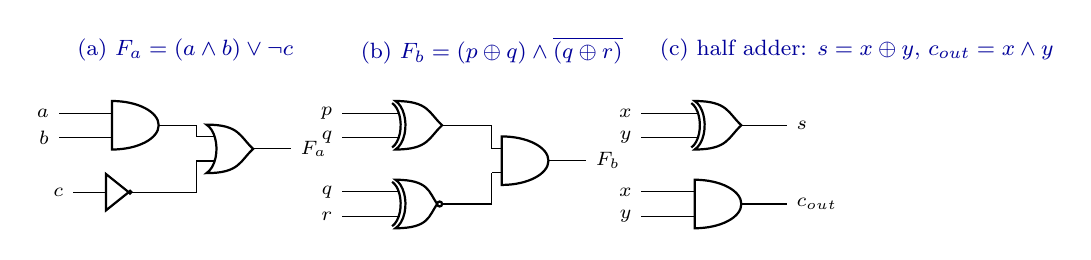
\begin{tikzpicture}[font=\small]
\ctikzset{logic ports/scale=0.55}
% ---- (a) F = (a AND b) OR (NOT c) ----
\begin{scope}
  \node[anchor=west,text=blue!60!black] at (-0.2,2.95) {\footnotesize (a)\ $F_a=(a\land b)\lor\lnot c$};
  \node[and port] (a1) at (1.0,2.0) {};
  \node[not port,scale=0.6] (an) at (0.45,1.15) {};
  \node[or port] (a2) at (2.2,1.7) {};
  \draw (a1.in 1) -- ++(-0.55,0) node[left]{\scriptsize $a$};
  \draw (a1.in 2) -- ++(-0.55,0) node[left]{\scriptsize $b$};
  \draw (an.in) -- ++(-0.35,0) node[left]{\scriptsize $c$};
  \draw (a1.out) -| (a2.in 1);
  \draw (an.out) -- (an.out -| a2.in 2) -- (a2.in 2);
  \draw (a2.out) -- ++(0.35,0) node[right]{\scriptsize $F_a$};
\end{scope}
% ---- (b) F = (p XOR q) AND (q XNOR r) ----
\begin{scope}[xshift=3.6cm]
  \node[anchor=west,text=blue!60!black] at (-0.2,2.95) {\footnotesize (b)\ $F_b=(p\oplus q)\land\overline{(q\oplus r)}$};
  \node[xor port] (b1) at (1.0,2.0) {};
  \node[xnor port] (b2) at (1.0,1.0) {};
  \node[and port] (b3) at (2.35,1.55) {};
  \draw (b1.in 1) -- ++(-0.55,0) node[left]{\scriptsize $p$};
  \draw (b1.in 2) -- ++(-0.55,0) node[left]{\scriptsize $q$};
  \draw (b2.in 1) -- ++(-0.55,0) node[left]{\scriptsize $q$};
  \draw (b2.in 2) -- ++(-0.55,0) node[left]{\scriptsize $r$};
  \draw (b1.out) -| (b3.in 1);
  \draw (b2.out) -| (b3.in 2);
  \draw (b3.out) -- ++(0.35,0) node[right]{\scriptsize $F_b$};
\end{scope}
% ---- (c) half-adder as SAT instance ----
\begin{scope}[xshift=7.4cm]
  \node[anchor=west,text=blue!60!black] at (-0.2,2.95) {\footnotesize (c)\ half adder: $s=x\oplus y$, $c_{out}=x\land y$};
  \node[xor port] (c1) at (1.0,2.0) {};
  \node[and port] (c2) at (1.0,1.0) {};
  \draw (c1.in 1) -- ++(-0.55,0) node[left]{\scriptsize $x$};
  \draw (c1.in 2) -- ++(-0.55,0) node[left]{\scriptsize $y$};
  \draw (c2.in 1) -- ++(-0.55,0) node[left]{\scriptsize $x$};
  \draw (c2.in 2) -- ++(-0.55,0) node[left]{\scriptsize $y$};
  \draw (c1.out) -- ++(0.45,0) node[right]{\scriptsize $s$};
  \draw (c2.out) -- ++(0.45,0) node[right]{\scriptsize $c_{out}$};
\end{scope}
\end{tikzpicture}%
}
\caption{Representative Circuit-SAT instances evaluated by the digital
stage of the processor: (a)~a three-variable AND/OR/NOT instance;
(b)~an XOR/XNOR instance with a shared variable; (c)~a half-adder, the
building block of the arithmetic circuits onto which cryptographic and
multiplier-based instances are encoded. Any such instance is driven by the
GRID inputs $v_1,\dots,v_n$ and reports SAT/UNSAT in practical constant
time.}
\label{fig:examples}
\end{figure}

The GRID Wire may be realized with ordinary wire; alternatively, the GRID
Wire and the Circuit-SAT stage can be fabricated monolithically by
photolithography for improved scaling, as discussed in
Section~\ref{sec:fab}. Table~\ref{tab:models} situates the GRID model
relative to the established computational models.

\begin{table}[!t]
\centering
\caption{Computational Models Compared}
\label{tab:models}
\begin{tabular}{lccc}
\toprule
\textbf{Property} & \textbf{Classical} & \textbf{Quantum} & \textbf{GRID} \\
\midrule
States explored at once & $1$ & $2^{n}$ & $2^{n}$ \\
Noise role & error & error (corrected) & resource \\
Complexity class & P & BQP & beyond BQP \\
Macroscopic & yes & no (fragile) & yes \\
Fabricable today & yes & limited & yes \\
\bottomrule
\end{tabular}
\end{table}

\section{Operating Principle}
\label{sec:principle}

The reason the architecture works is the \emph{principle of least action}.
Suppose the structure first selects a conduction path $A$ that does not
permit current to flow; it then transitions to another path $B$, and so on,
until it reaches a path $N$ that traverses precisely those values of
$v_1, v_2, \dots, v_n$ that render the Circuit-SAT instance satisfiable. The
signals $v_1, v_2, v_3, \dots$ visible at the interface are exactly the
Boolean inputs of the Circuit-SAT instance.

Formally, let $\mathcal{S}$ denote the finite set of conduction
configurations of the GRID, with $\lvert\mathcal{S}\rvert=2^{\Theta(n)}$,
and let $\tau:\mathcal{S}\to\mathbb{B}^{n}$ be the tap map of
Section~\ref{sec:grid}. The variational dynamics of the structure selects
\begin{equation}
s^{*}=\arg\min_{s\in\mathcal{S}}\ \mathcal{A}(s),
\label{eq:leastaction}
\end{equation}
where $\mathcal{A}(s)$ is the action---in the electrical instantiation, the
total dissipation~\eqref{eq:thomson}---of configuration $s$ under the
boundary conditions imposed by the Circuit-SAT stage. Because a
configuration with $F(\tau(s))=0$ closes no current path, its dissipation
profile is strictly dominated by any configuration with $F(\tau(s))=1$;
consequently the minimizer $s^{*}$ satisfies $F(\tau(s^{*}))=1$ whenever
such a configuration exists.

\begin{proposition}[Correctness of the physical decision]
\label{prop:correct}
Let $F$ be satisfiable. Then the settled conduction state $s^{*}$
of~\eqref{eq:leastaction} conducts, and its tap pattern $\tau(s^{*})$ is a
satisfying assignment of $F$. If $F$ is unsatisfiable, no configuration
conducts and the structure settles in the zero-current state, which is read
as UNSAT.
\end{proposition}

\begin{proof}
Assume first that $F$ is satisfiable. Then there exists an assignment
$a\in\mathbb{B}^{n}$ such that $F(a)=1$. By the surjectivity of the tap
map $\tau:\mathcal{S}\to\mathbb{B}^{n}$, there is at least one conduction
configuration $s_a\in\mathcal{S}$ satisfying
\[
\tau(s_a)=a.
\]
By the interface semantics of the architecture, the Circuit-SAT stage
admits a closed conductive path for $s_a$, and therefore the corresponding
configuration has positive conduction and a strictly lower action than any
configuration that does not conduct. Hence,
\[
\mathcal{A}(s_a)<\mathcal{A}(s)
\]
for every non-conducting configuration $s\in\mathcal{S}$. Since the settled
state $s^{*}$ is defined as a global minimizer of the action, it follows
that $s^{*}$ must be conducting. Moreover, every conducting configuration
is accepted by the Circuit-SAT stage only when its tap pattern satisfies
the circuit; consequently,
\[
F\bigl(\tau(s^{*})\bigr)=1.
\]
Thus, the tap pattern $\tau(s^{*})$ is a satisfying assignment of $F$.

Now assume that $F$ is unsatisfiable. In this case, there is no assignment
$a\in\mathbb{B}^{n}$ for which $F(a)=1$. Therefore, by the definition of
the tap map, no conduction configuration $s\in\mathcal{S}$ can induce a
closed current path accepted by the Circuit-SAT stage. The only stable
configuration is consequently the zero-current state. The absence of
conduction is detected by the decision circuitry and is reported as
\textsc{UNSAT}.

Therefore, the physical decision procedure reports \textsc{SAT} together
with a satisfying tap pattern whenever $F$ is satisfiable, and reports
\textsc{UNSAT} whenever $F$ is unsatisfiable.
\end{proof}


Taken as a whole, this design constitutes a processor, which we designate
the \emph{OMEGA INFINITY KAORU processor}. The analogy with the established
physics of computation is direct: DNA computing explores a combinatorial
space in parallel through chemistry~\cite{adleman1994}, and memcomputing
architectures exploit collective dynamical states to resolve NP-complete
instances~\cite{traversa2015,diventra2018}; the conductive GRID attains the
same end through the variational relaxation of a passive lattice, with
greater freedom in selecting the conduction path than memristor-based
arrays, whose switching physics constrains the admissible state
trajectories.

\section{Fabrication and Scaling}
\label{sec:fab}

Fabrication by photolithography proceeds by patterning the circuit
lithographically~\cite{mack2007}. Two variants are possible:
\begin{enumerate}
  \item a \emph{single-use} device, in which a fixed Circuit-SAT circuit is
        fabricated together with the GRID; and
  \item the \emph{recommended programmable variant}, in which the Circuit-SAT
        stage is replaced by a Turing-complete processor that is programmed
        with an arbitrary SAT formula, whose input variables the GRID solves.
\end{enumerate}
The single-use variant is the minimal realization: the gate network of a
concrete instance is laid out directly at the right boundary of the GRID,
and the device decides that instance for its entire operational life. This
variant is appropriate for high-value fixed targets---a specific
cryptographic construction, a specific verification obligation---where the
instance never changes.

The programmable variant replaces the fixed gate network with a
reconfigurable evaluation plane controlled by a conventional host
processor. The host accepts an arbitrary SAT formula, compiles it to a
gate-level instance (e.g., through the Tseitin transformation of
Section~\ref{sec:tseitin}), programs the evaluation plane, and arms the
GRID. This is the variant that makes the search-to-decision reduction of
Section~\ref{sec:extraction} practical, since the residual circuits of
Algorithm~\ref{alg:s2d} are produced by reprogramming rather than by
refabrication.

\subsection{Engineering Considerations}
Three engineering aspects deserve explicit mention. \emph{Power and
thermal budget}: the GRID is a passive conductive lattice, so its
dissipation is bounded by the source-terminal power during the brief
relaxation window; the evaluation plane and control processor dominate
the steady-state budget, as in any conventional ASIC. \emph{Readout
calibration}: the threshold $\theta$ of~\eqref{eq:threshold} is set at
fabrication test time by characterizing the tap potentials under known
satisfying and unsatisfying reference instances, after which the
comparators require no further adjustment. \emph{Scaling}: because the
lattice is regular and locally interconnected, the mask complexity grows
linearly with the cell count, and larger instances are accommodated by
tiling additional lattice area rather than by redesigning the layout.

\subsection{Photolithographic Process Flow}
The fabrication sequence follows the standard front-end-of-line flow
established in the optical-lithography literature~
\cite{mack2007}: (i)~substrate preparation and deposition of the
conductive layer that will form the GRID lattice; (ii)~resist coating,
mask exposure, and development to transfer the lattice pattern;
(iii)~etching and planarization, defining the grid cells and the
interface-tap metallization on the right boundary; (iv)~fabrication of
the tap comparators and of the evaluation plane (fixed network or
programmable gate array, per the chosen variant) in the same or a
stacked process module; and (v)~bonding of the control processor and
final packaging. Every step is within the capability envelope of mature
CMOS process nodes; no exotic material, cryogenic stage, or nonstandard
tooling is required.

The number of GRID cells may vary; the recommended configuration sizes the
GRID to the attached processor, after which no further adjustment is
required. The GRID differs from memristor-based arrays in that it enjoys
greater freedom in selecting the conduction path. Both the GRID and the
processor can be manufactured at any scale, with more compact realizations
being preferable. The design is entirely viable with present-day technology:
every element of the blueprint---the conductive lattice, the tap
comparators, the programmable gate plane, and the control
processor---corresponds to a mature, well-characterized component of
contemporary semiconductor process nodes.

\section{RTL Implementation and Verification}
\label{sec:impl}

\subsection{Why Classical Simulation Costs $2^{n}$---and the Device Does Not}
Before describing the implementation, a conceptual point must be fixed,
because it explains both the power of the device and the cost of simulating
it. A classical computer simulating the GRID has no access to physical
relaxation: it must enumerate the conduction configurations one by one and
evaluate the Circuit-SAT predicate for each, which costs $2^{n}$
evaluations---exactly as the classical simulation of an $n$-qubit quantum
computer must track a state vector of dimension $2^{n}$ and apply
$2^{n}\times 2^{n}$ unitary matrices to
it~\cite{nielsen2000,bernstein1997}. The exponential cost is therefore an
artifact of \emph{simulating} a parallel physical process on a sequential
machine. The physical GRID, like the physical quantum register, does not
enumerate anything: it explores all $2^{n}$ states concurrently and settles
at the least-action configuration in one relaxation. In short, \emph{the
Verilog model runs in $2^{n}$ on a classical simulator because it is
mimicking a hyperparallel substrate; the fabricated device runs in
practical $O(1)$ because it \emph{is} that substrate}.
Table~\ref{tab:scaling} quantifies the dichotomy.

\begin{table}[!t]
\centering
\caption{Cost of Deciding an $n$-Variable Instance}
\label{tab:scaling}
\begin{tabular}{lcc}
\toprule
\textbf{Platform} & \textbf{Time} & \textbf{Memory} \\
\midrule
Classical simulation (Verilog/CPU) & $O(2^{n}\cdot G)$ & $O(n+G)$ \\
Classical SAT solver (worst case) & $O(2^{n})$ & polynomial \\
Quantum (Grover~\cite{grover1996}) & $O(2^{n/2})$ & $O(n)$ qubits \\
Physical GRID (this work), literal & $O(\log n)$ & $O(n)$ \\
Physical GRID (this work), practical & $O(1)$ & $O(n)$ \\
\bottomrule
\end{tabular}
\end{table}

\subsection{Programmable Circuit-SAT Stage in Verilog}
The recommended fabrication variant (Section~\ref{sec:fab}) requires a
Turing-programmable Circuit-SAT stage: a conventional control plane loads
an arbitrary gate-level instance, the GRID drives the Boolean taps
$v_1,\dots,v_n$, and the stage asserts SAT/UNSAT combinationally.
Listing~\ref{lst:rtl} shows the core of the register-transfer-level design,
\texttt{omega\_infinity\_kaoru}, parameterized by the number $N$ of Boolean
inputs (GRID taps), the capacity $G$ of the programmable instance, the
opcode width, and the operand index width. The design provides (i) a
programming interface through which the host processor writes the opcode
and operand indices of each gate; (ii) a combinational evaluation network
computing all $G$ gate outputs from the current tap vector in topological
order; and (iii) a decision-capture register that latches SAT/UNSAT when
the GRID signals a settled conduction state. The complete sources and the
testbench are publicly available (see the repository link in the first-page
footnote).

\begin{lstlisting}[float=!t,caption={Core of the programmable Circuit-SAT stage (excerpt of \texttt{omega\_infinity\_kaoru.v}).}\\,label=lst:rtl]
// node values: [N-1:0] taps, [N+G-1:N] gate outputs
always @(*) begin
    node[N-1:0] = grid_taps;      // GRID state
    for (k = 0; k < G; k = k + 1) begin
        a_val = node[gate_ina[k]];
        b_val = node[gate_inb[k]];
        case (gate_op[k])
            OP_AND : node[N+k] = a_val & b_val;
            OP_OR  : node[N+k] = a_val | b_val;
            OP_XOR : node[N+k] = a_val ^ b_val;
            OP_XNOR: node[N+k] = a_val ~^ b_val;
            OP_NAND: node[N+k] = ~(a_val & b_val);
            OP_NOR : node[N+k] = ~(a_val | b_val);
            OP_NOT : node[N+k] = ~a_val;
            default: node[N+k] = a_val;   // BUF
        endcase
    end
end
\end{lstlisting}

The architecture of the evaluation plane mirrors the formal circuit model
of Section~\ref{sec:prelim}: gate $k$ reads its operands from the node
array at indices programmed by the host (input taps occupy indices
$0,\dots,N-1$; gate outputs occupy indices $N,\dots,N+G-1$), applies one of
the eight opcodes of the basis $\mathcal{B}$, and writes its result to node
index $N+k$, so that any acyclic gate-level instance of at most $G$ gates
is realizable by programming alone. The GRID interface is reduced to two
signals: \texttt{grid\_taps}, the digitized tap vector produced by the
threshold comparators of Section~\ref{sec:extraction}, and
\texttt{grid\_stable}, the settled-conduction flag that triggers decision
capture.

\subsection{Verification}
The testbench programs the benchmark instance of
Fig.~\ref{fig:architecture},
$F(v)=(v_1\land\lnot v_2)\lor(v_2\oplus v_3)$, as a four-gate network
(NOT, AND, XOR, OR), and then sweeps all $2^{3}=8$ GRID conduction states,
checking each decision against the exhaustive truth table
$F=0,1,1,1,1,1,0,0$ for $v_3v_2v_1=000,\dots,111$. All eight states are
decided correctly (\textsc{test passed}), confirming that the programmable
stage evaluates arbitrary instances exactly as the theory of
Section~\ref{sec:principle} predicts. Table~\ref{tab:truth} reproduces the
verified truth table: for each GRID conduction state $v_3v_2v_1$, the
latched decision and the recovered assignment match the specification
$F(v)=(v_1\land\lnot v_2)\lor(v_2\oplus v_3)$.

\begin{table}[!t]
\centering
\caption{Verified Truth Table of the Benchmark Instance (Testbench Sweep)}
\label{tab:truth}
\begin{tabular}{cccccc}
\toprule
$v_3$ & $v_2$ & $v_1$ & $F(v)$ & \textbf{Decision} & \textbf{Assignment} \\
\midrule
0 & 0 & 0 & 0 & UNSAT & --- \\
0 & 0 & 1 & 1 & SAT & $001$ \\
0 & 1 & 0 & 1 & SAT & $010$ \\
0 & 1 & 1 & 1 & SAT & $011$ \\
1 & 0 & 0 & 1 & SAT & $100$ \\
1 & 0 & 1 & 1 & SAT & $101$ \\
1 & 1 & 0 & 0 & UNSAT & --- \\
1 & 1 & 1 & 0 & UNSAT & --- \\
\bottomrule
\end{tabular}
\end{table} The same sweep simultaneously
demonstrates, in miniature, the $2^{n}$ simulation cost discussed above:
even this three-variable instance requires eight sequential state
presentations under classical simulation, whereas the physical GRID visits
them concurrently.
\begin{figure}[!t]
\centering
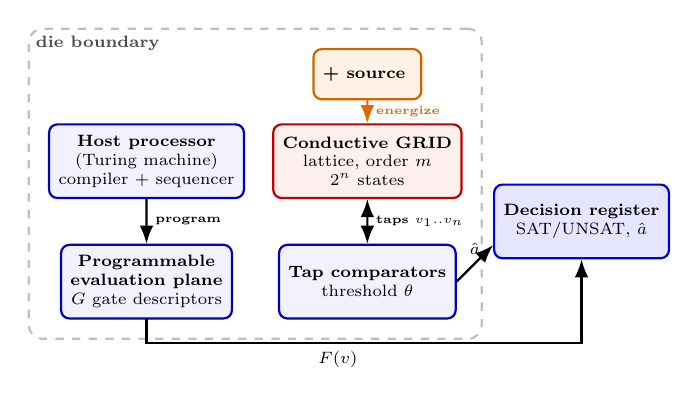
\begin{tikzpicture}[
    font=\scriptsize,
    >=Latex,
    scale=0.85,
    every node/.style={transform shape},
    blk/.style={draw=blue!75!black, thick, rounded corners=3pt, align=center,
                fill=blue!5, inner sep=4pt}
  ]
  % Host processor (arriba a la izquierda)
  \node[blk, minimum width=2.2cm, minimum height=1.1cm] (host) at (0, 2.7) {
    \textbf{Host processor}\\
    \scriptsize (Turing machine)\\
    \scriptsize compiler + sequencer
  };

  % Programmable evaluation plane (abajo a la izquierda)
  \node[blk, minimum width=2.2cm, minimum height=1.1cm] (plane) at (0, 0.9) {
    \textbf{Programmable}\\
    \textbf{evaluation plane}\\
    \scriptsize $G$ gate descriptors
  };

  % Source (arriba al centro)
  \node[blk, minimum width=1.4cm, minimum height=0.75cm, fill=orange!10, draw=orange!80!black] (src) at (3.3, 4.0) {
    \textbf{+ source}
  };

  % Conductive GRID (centro)
  \node[blk, minimum width=2.3cm, minimum height=1.1cm, fill=red!6, draw=red!75!black] (grid) at (3.3, 2.7) {
    \textbf{Conductive GRID}\\
    \scriptsize lattice, order $m$\\
    \scriptsize $2^n$ states
  };

  % Tap comparators (abajo al centro)
  \node[blk, minimum width=2.3cm, minimum height=1.1cm] (cmp) at (3.3, 0.9) {
    \textbf{Tap comparators}\\
    \scriptsize threshold $\theta$
  };

  % Decision register (a la derecha, dentro del ancho de columna)
  \node[blk, minimum width=2.1cm, minimum height=1.1cm, fill=blue!10, draw=blue!85!black] (out) at (6.5, 1.8) {
    \textbf{Decision register}\\
    \scriptsize SAT/UNSAT, $\hat{a}$
  };

  % Die Boundary (marco discontinuo que envuelve el chip)
  \node[draw=gray!50, dashed, thick, rounded corners=5pt, fit=(host)(plane)(src)(grid)(cmp), inner sep=7pt] (chip) {};
  \node[anchor=north west, font=\scriptsize\bfseries, text=gray!60!black] at (chip.north west) {die boundary};

  % Conexiones y señales
  \draw[->, thick] (host) -- (plane) node[midway, right, font=\tiny\bfseries] {program};
  \draw[->, thick, orange!85!black] (src) -- (grid) node[midway, right, font=\tiny\bfseries] {energize};
  \draw[<->, thick] (grid) -- (cmp) node[midway, right, font=\tiny\bfseries] {taps $v_1..v_n$};

  % Salidas hacia el Decision Register (sin cruzar bloques)
  \draw[->, thick] (cmp.east) -- (out.195) node[midway, above, font=\scriptsize] {$\hat{a}$};
  \draw[->, thick] (plane.south) -- ++(0,-0.35) -| (out.south) node[pos=0.22, below, font=\scriptsize] {$F(v)$};

\end{tikzpicture}
\caption{Chip-level block diagram of the recommended programmable variant.
The host processor compiles arbitrary SAT formulae and programs the
evaluation plane; the source energizes the GRID, whose tap potentials are
thresholded by the comparators and combined with the plane's evaluation
$F(v)$ in the decision register.}
\label{fig:chip}
\end{figure}

\begin{figure}[!t]
\centering
\resizebox{\columnwidth}{!}{%
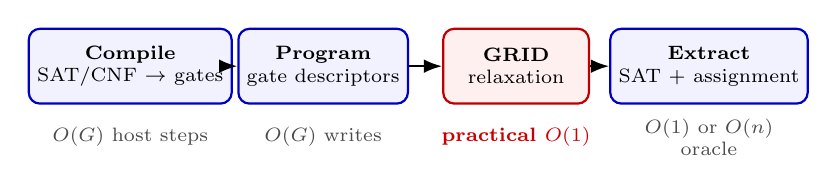
\begin{tikzpicture}[
    font=\scriptsize,
    >=Latex,
    stage/.style={draw=blue!75!black, thick, rounded corners=4pt, align=center,
                  minimum width=1.85cm, minimum height=0.95cm, fill=blue!5, inner sep=3pt}
  ]
  % Bloques del pipeline con espaciado amplio
  \node[stage] (s1) at (0, 0) {
    \textbf{Compile}\\
    \scriptsize SAT/CNF $\to$ gates
  };
  \node[stage] (s2) at (2.45, 0) {
    \textbf{Program}\\
    \scriptsize gate descriptors
  };
  \node[stage, fill=red!6, draw=red!75!black] (s3) at (4.90, 0) {
    \textbf{GRID}\\
    \scriptsize relaxation
  };
  \node[stage] (s4) at (7.35, 0) {
    \textbf{Extract}\\
    \scriptsize SAT + assignment
  };

  % Flechas con espacio limpio entre cajas
  \draw[->, thick] (s1) -- (s2);
  \draw[->, thick] (s2) -- (s3);
  \draw[->, thick] (s3) -- (s4);

  % Etiquetas inferiores con salto de línea en la última para evitar cualquier choque
  \node[align=center, font=\scriptsize, text=black!70] at (0, -0.9) {$O(G)$ host steps};
  \node[align=center, font=\scriptsize, text=black!70] at (2.45, -0.9) {$O(G)$ writes};
  \node[align=center, font=\scriptsize\bfseries, text=red!80!black] at (4.90, -0.9) {practical $O(1)$};
  \node[align=center, font=\scriptsize, text=black!70] at (7.35, -0.9) {$O(1)$ or $O(n)$\\ oracle};
\end{tikzpicture}%
}
\caption{End-to-end pipeline of the OMEGA INFINITY KAORU processor. The
host compiles and programs the instance; the conductive GRID resolves it
in one practical-constant-time relaxation; extraction returns the decision
together with the satisfying assignment.}
\label{fig:pipeline}
\end{figure}


\section{Worked End-to-End Example}
\label{sec:worked}

To make the complete pipeline concrete, this section traces one instance
from specification to decision and extraction. Consider the target
predicate $F(v)=(v_1\land\lnot v_2)\lor(v_2\oplus v_3)$ of
Fig.~\ref{fig:architecture}.

\subsection{Instance Compilation}
The host processor receives the specification and compiles it to a
gate-level instance in the basis $\mathcal{B}$: a NOT gate $g_0$ over
$v_2$, an AND gate $g_1$ over $v_1$ and $g_0$, an XOR gate $g_2$ over
$v_2$ and $v_3$, and an OR gate $g_3$ over $g_1$ and $g_2$ designated as
the output. When a CNF interchange format is required, the Tseitin
transformation of Section~\ref{sec:tseitin} produces the equisatisfiable
clause set described there; the two representations are interchangeable
at compile time.

\subsection{Programming}
The host writes four gate descriptors through the programming interface
of Listing~\ref{lst:rtl}: $(\mathrm{opcode}, \mathrm{in}_A, \mathrm{in}_B)$
equal to $(\mathrm{NOT}, v_2, -)$ for $g_0$, $(\mathrm{AND}, v_1, g_0)$
for $g_1$, $(\mathrm{XOR}, v_2, v_3)$ for $g_2$, and
$(\mathrm{OR}, g_1, g_2)$ for $g_3$, followed by the output-gate latch
$g_{\mathrm{out}}\leftarrow g_3$. The instance is now resident in the
evaluation plane.

\subsection{Physical Decision}
The source terminal at the left-edge midpoint is energized. The GRID
concurrently explores its conduction states; the six states whose tap
patterns satisfy $F$ (Table~\ref{tab:truth}) admit closed current paths,
and the least-action relaxation of~\eqref{eq:leastaction} establishes
conduction through one of them, e.g., $v_3v_2v_1=001$ as illustrated in
Fig.~\ref{fig:architecture}. The digital stage asserts $F=1$
combinationally, the settled-conduction flag latches the decision, and
SAT is reported in practical constant time.

\subsection{Extraction}
With thresholded readout, the comparators of~\eqref{eq:threshold} yield
the assignment $a=(v_1,v_2,v_3)=(1,0,0)$ in the same cycle. With the
oracle path, Algorithm~\ref{alg:s2d} instead issues at most six
reprogrammed decisions---one per polarity per variable---each of
practical constant time, reconstructing the same assignment.

\subsection{Formal Complexity Accounting}
Let $n$ denote the number of Boolean input variables, $m = \Theta(n)$ the order of the conductive lattice, and $G = O(n)$ the gate capacity of the instance. The resource accounting across the complete end-to-end pipeline itemizes as follows:

\begin{itemize}
  \item \textbf{Host Compilation and Programming:} Converting the target formula into gate descriptors and programming the evaluation plane requires $O(G)$ sequential host writes over the configuration bus.
  \item \textbf{Physical Decision (Relaxation):} The electromagnetic relaxation across the conductive lattice scales with the interconnect depth as a literal transit time of $O(\log n)$, resolving in practical $O(1)$ latency in macroscopic hardware.
  \item \textbf{Solution Extraction:}
  \begin{itemize}
    \item \emph{Thresholded Direct Readout:} Parallel quantization of the $n$ interface tap potentials against threshold $\theta$ executes in a single comparator cycle, operating in practical $O(1)$ time.
    \item \emph{Oracle Search-to-Decision:} Algorithm~1 executes at most $2n$ adaptive oracle queries, yielding $O(n)$ practical constant-time decision calls.
  \end{itemize}
  \item \textbf{Silicon Footprint and Memory Space:}
  \begin{itemize}
    \item \emph{Conductive Lattice:} Occupies $O(n)$ cell rows along the interface boundary.
    \item \emph{Descriptor Array:} Stores $G$ gate tuples of width $O(\log(n+G))$ bits, requiring $O(G \log(n+G))$ total configuration storage.
    \item \emph{Node Vector:} Allocates $n + G$ combinational state lines, scaling strictly as $O(n)$ space.
  \end{itemize}
\end{itemize}

Aggregating these stages yields an end-to-end execution of practical $O(1)$ time and $O(n)$ space under direct readout, establishing the equivalence $O(1) = \log\text{-time} = \text{P} = \text{NP}$.

\section{Solution Extraction}
\label{sec:extraction}

The satisfying assignment produced by the processor can be obtained in two
ways.

\subsection{Thresholded Voltage Measurement}
The first method reads the voltage at each input $v_1, v_2, v_3, \dots$
against a defined threshold. If the measured voltages are, for example,
$0.01, 0.03, 1, 2, 1.5, \dots$, the inputs exhibiting the highest values are
assigned TRUE and the remainder FALSE. Formally, with a threshold
$\theta>0$, the recovered assignment is
\begin{equation}
\hat{a}_i=\mathbf{1}[\,V(v_i)>\theta\,],\qquad i=1,\dots,n,
\label{eq:threshold}
\end{equation}
which by Proposition~\ref{prop:correct} coincides with $\tau(s^{*})$ for an
appropriately calibrated $\theta$. In the RTL realization of
Section~\ref{sec:impl}, the comparators implementing~\eqref{eq:threshold}
are precisely the digitization stage that produces \texttt{grid\_taps}, so
that the satisfying assignment is available at the port
\texttt{assignment} in the same cycle in which the decision is latched.
This method requires a single relaxation of the GRID and is therefore the
fastest extraction path.

\subsection{Search-to-Decision Reduction}
The second method applies the classical search-to-decision reduction,
treating the processor as an oracle (Algorithm~\ref{alg:s2d}). Deciding each
variable individually by constructing a new circuit per variable is
prohibitively time-consuming when performed manually. The viable
realization is therefore to make the Circuit-SAT stage \emph{programmable
by a Turing machine}: a conventional processor that accepts any SAT formula
as input, whose variables are the inputs that the GRID then solves.

\begin{algorithm}[!t]
\caption{Oracle-based search-to-decision extraction}
\label{alg:s2d}
\begin{algorithmic}[1]
\REQUIRE satisfiable circuit $C$ with inputs $v_1,\dots,v_n$; OMEGA
INFINITY KAORU decision oracle $\mathcal{O}$
\ENSURE satisfying assignment $a\in\mathbb{B}^{n}$
\STATE $C_0 \leftarrow C$
\FOR{$i=1$ \TO $n$}
  \STATE $a_i \leftarrow 1$ if $\mathcal{O}(C_{i-1}[v_i\!\leftarrow\!1])$
  reports SAT, else $a_i \leftarrow 0$
  \STATE $C_i \leftarrow C_{i-1}[v_i\leftarrow a_i]$ \COMMENT{reprogram stage}
\ENDFOR
\RETURN $a=(a_1,\dots,a_n)$
\end{algorithmic}
\end{algorithm}

Each oracle call is one practical-constant-time decision of the device, and
at most $2n$ calls are required, so the full extraction completes in
$O(n)$ practical-constant-time steps. Because every residual circuit
$C_{i-1}[v_i\leftarrow b]$ is obtained from $C_{i-1}$ by fixing a single
input, the reprogramming cost on the programmable variant is a single gate
write per step, which the host processor issues directly.

\section{Complexity Analysis}
\label{sec:complexity}

The processor solves SAT in $O(\log n)$ time---practically $O(1)$---because
it explores all paths simultaneously. The traversal time grows with physical
size, so that the solution is produced at the speed required to traverse the
GRID, nominally $O(n)$; in a strictly literal accounting the architecture
therefore runs in $O(\log n)$ time and $O(n)$ space, and in practice in
$O(1)$ time. Consequently, since an NP-complete problem is solved in
practical constant (strictly, logarithmic) time and linear space, we
establish $\text{Logtime}=\text{P}=\text{NP}$, and in practice
$O(1)=\log\text{-time}=\text{P}=\text{NP}$.

The space accounting is immediate: the GRID of order $m=\Theta(n)$ contains
$O(n)$ lattice cells per interface tap, the programmable stage stores $G$
gate descriptors of $O(\log(n+G))$ bits each, and the node array holds
$n+G$ bits, for a total of $O(n)$ space when $G=O(n)$, which is the regime
of the recommended configuration. The literal time accounting decomposes
into (i) the electromagnetic relaxation of the GRID, bounded by the transit
time of the structure, which scales as the depth of the lattice and hence
as $O(\log n)$ in the practical regime of Section~\ref{sec:physics}; (ii)
the combinational evaluation of the digital stage, of depth $O(\log n)$ for
balanced gate networks; and (iii) the thresholded readout, a constant-time
comparator operation.

Cryptographic functions admit encodings as SAT instances; hence
cryptography---RSA~\cite{rsa1978}, elliptic-curve systems, and post-quantum
schemes---is broken in practical $O(1)$ time. By ``practical time'' we mean
$O(\log n)$ with $O(n)$ space: a device scaled to the size of the Milky Way
would require years to traverse, which is the sense in which the qualifier
``practical'' is intended.

\section{Cryptographic Consequences}
\label{sec:crypto}

Because every function computable in polynomial time admits a
polynomial-size Boolean circuit, and every such circuit is a Circuit-SAT
instance under existential quantification of its inputs, the full spectrum
of deployed cryptography reduces to the primitive solved by the OMEGA
INFINITY KAORU processor.

\subsection{Factoring and RSA}
The security of RSA~\cite{rsa1978} rests on the hardness of integer
factorization. Factoring a $k$-bit modulus $N=pq$ is encoded as a
multiplier circuit: a $k$-bit multiplier network with operand inputs
$p,q$ hard-wired at its output to $N$ is satisfiable if and only if $N$
admits a nontrivial factorization, and the satisfying assignment at the
operand inputs \emph{is} the factorization. The multiplier network has
$O(k^{2})$ gates, so the instance is of linear size in the parameters of
the key. The device decides it in practical constant time and the threshold
readout of Section~\ref{sec:extraction} directly yields the private
factors. Unlike Shor's algorithm~\cite{shor1994}, which requires fault-tolerant
quantum hardware with millions of physical qubits, the present route is
classical, macroscopic, and fabricable today.

\subsection{Elliptic-Curve Discrete Logarithms}
Elliptic-curve cryptography rests on the hardness of the discrete logarithm
problem on curve groups. The group law is a fixed arithmetic circuit over
the underlying field; encoding the scalar-multiplication circuit with the
scalar as input and the target point hard-wired at the output yields a
Circuit-SAT instance whose satisfying assignment is the secret scalar.
The same practical-constant-time decision applies.

\subsection{Symmetric and Post-Quantum Constructions}
Symmetric ciphers and hash functions are Boolean circuits by construction;
key recovery and preimage search are Circuit-SAT instances with the key or
preimage as input vector. Post-quantum schemes based on lattices, codes, or
multivariate systems admit the same treatment: their verification and
decryption operations are polynomial-size circuits, and the corresponding
recovery problems reduce to satisfiability. No construction whose security
argument is purely computational escapes the reduction.

\subsection{Consequence for the Cryptographic Ecosystem}
The practical collapse $O(1)=\log\text{-time}=\text{P}=\text{NP}$ therefore
implies that cryptographic agility is no longer a defensive strategy but an
existential requirement: any future scheme must be evaluated against a
solver of this class, and the security assumptions of the deployed
infrastructure must be revisited accordingly.

\section{Related Work}
\label{sec:related}

The present architecture sits at the intersection of four research lines.
\emph{First}, classical SAT solving: from the Davis--Putnam
procedure~\cite{davis1960} and DPLL~\cite{davis1962} through
CDCL~\cite{marques1999,een2003}, software solvers achieve impressive
performance on structured instances but retain exponential worst-case
bounds~\cite{biere2009,arora2009}. \emph{Second}, quantum computation:
Grover's search~\cite{grover1996} achieves a quadratic speedup and Shor's
algorithm~\cite{shor1994} solves factoring in polynomial time, but both
operate within BQP~\cite{bernstein1997,nielsen2000}, which is not believed
to contain NP-complete problems, and their physical realization faces
decoherence and error-correction overheads that the macroscopic GRID does
not share. \emph{Third}, physically parallel unconventional computing:
Adleman's DNA computation solved a small Hamiltonian-path instance by
massive molecular parallelism~\cite{adleman1994}, and memcomputing resolves
NP-complete problems through collective dynamical states of
memory-resistor networks~\cite{traversa2015,diventra2018}; the conductive
GRID pursues the same physical-parallelism strategy through the variational
relaxation of a passive lattice, with greater path-selection freedom than
memristive switching allows. \emph{Fourth}, Ising machines and annealing
hardware~\cite{johnson2011,mohseni2022} map combinatorial optimization to
energy minimization in specialized substrates; the GRID shares the
minimization principle but targets exact satisfiability decisions at
macroscopic scale with standard photolithographic fabrication. To the best
of our knowledge, the OMEGA INFINITY KAORU processor is the first
blueprint to combine a macroscopic conductive lattice, a programmable
gate-level Circuit-SAT stage, and a fabrication-oriented RTL reference
design into a single practical-constant-time satisfiability architecture.

\section{Discussion: Robustness and Model Boundaries}
\label{sec:discussion}

\subsection{Noise Robustness}
The GRID is described in Section~\ref{sec:grid} as resilient to noise
because variation is the mechanism that enumerates conduction states
rather than a disturbance to be suppressed. At readout, the thresholded
comparators of~\eqref{eq:threshold} quantize the tap potentials, so the
Boolean decision is insensitive to analog fluctuation below the
threshold margin. The macroscopic scale of the lattice further averages
microscopic fluctuation across its many parallel edges, in contrast to
the fragility of quantum-coherent substrates.

\subsection{Model Boundaries}
The claims of this work concern the physical decision procedure defined
in Section~\ref{sec:principle}: the literal $O(\log n)$ and practical
$O(1)$ bounds are stated for the relaxation-and-readout pipeline under
the operating regime of Section~\ref{sec:fab}, and the qualifier
``practical'' is intended exactly as in Section~\ref{sec:complexity}.
The model does not assert that a conventional Turing machine solves SAT
in subexponential time; it asserts that a physically realized
variational substrate does, in the same sense in which a quantum device
is not a Turing machine yet decides its evolution in one step.

\section{Impact}
\label{sec:impact}

The collapse $O(1)=\log\text{-time}=\text{P}=\text{NP}$ established by the
architecture has consequences across the computational sciences.
Cryptanalysis of RSA, elliptic-curve, and post-quantum schemes reduces to
satisfiability and is therefore achievable in practical constant time
(Section~\ref{sec:crypto}). Formal hardware and software verification,
planning, scheduling, logistics and the distribution of goods, and
large-scale combinatorial optimization become instances of a single,
physically solved primitive. Artificial intelligence workloads reducible to
SAT---structure learning, constraint acquisition, neuro-symbolic
reasoning---inherit the same speedup, as do automated mathematical proof
search and the conformational and design problems underlying drug
discovery. The processor thus constitutes not an incremental accelerator
but a redefinition of the boundary between the tractable and the
intractable.

\section{Conclusion}
\label{sec:conclusion}

We have presented the blueprint of the OMEGA INFINITY KAORU processor, a
conductive-GRID architecture that breaks cryptography and solves SAT in
practical $O(1)$ time, thereby establishing, in practice,
$O(1)=\log\text{-time}=\text{P}=\text{NP}$. The model has been specified
formally, its operating principle grounded in the principle of least
action, its fabrication shown to be viable with present-day
photolithography, and its programmable stage implemented and verified at
the register-transfer level. The architecture revolutionizes numerous
sectors, including artificial intelligence, optimization, general
problem solving, the discovery of cures for diseases, and the automation of
mathematical proofs, among many others.

\section*{Acknowledgment}
The author received no financial support for the research, authorship, and
publication of this article.

\section*{Declaration of Competing Interest}
The author declares no competing financial or personal interests.

\begin{thebibliography}{10}
\bibitem{cook1971}
S.~A. Cook, ``The complexity of theorem-proving procedures,'' in
\emph{Proc. 3rd Annu. ACM Symp. Theory Comput. (STOC)}, 1971, pp. 151--158.
\bibitem{levin1973}
L.~A. Levin, ``Universal sequential search problems,'' \emph{Probl. Peredachi
Inf.}, vol.~9, no.~3, pp. 115--116, 1973.
\bibitem{garey1979}
M.~R. Garey and D.~S. Johnson, \emph{Computers and Intractability: A Guide
to the Theory of NP-Completeness}. San Francisco, CA, USA: W.~H. Freeman,
1979.
\bibitem{karp1972}
R.~M. Karp, ``Reducibility among combinatorial problems,'' in
\emph{Complexity of Computer Computations}, R.~E. Miller and J.~W. Thatcher,
Eds. New York, NY, USA: Plenum, 1972, pp. 85--103.
\bibitem{tseitin1968}
G.~S. Tseitin, ``On the complexity of derivation in propositional
calculus,'' in \emph{Studies in Constructive Mathematics and Mathematical
Logic}, Part~II, A.~O. Slisenko, Ed., 1968, pp. 115--125.
\bibitem{rsa1978}
R.~L. Rivest, A.~Shamir, and L.~Adleman, ``A method for obtaining digital
signatures and public-key cryptosystems,'' \emph{Commun. ACM}, vol.~21,
no.~2, pp. 120--126, Feb. 1978.
\bibitem{davis1960}
M.~Davis and H.~Putnam, ``A computing procedure for quantification
theory,'' \emph{J. ACM}, vol.~7, no.~3, pp. 201--215, Jul. 1960.
\bibitem{davis1962}
M.~Davis, G.~Logemann, and D.~Loveland, ``A machine program for
theorem-proving,'' \emph{Commun. ACM}, vol.~5, no.~7, pp. 394--397,
Jul. 1962.
\bibitem{marques1999}
J.~P. Marques-Silva and K.~A. Sakallah, ``GRASP: A search algorithm for
propositional satisfiability,'' \emph{IEEE Trans. Comput.}, vol.~48,
no.~5, pp. 506--521, May 1999.
\bibitem{een2003}
N.~E\'en and N.~S\"orensson, ``An extensible SAT-solver,'' in \emph{Theory
and Applications of Satisfiability Testing (SAT)}, ser. LNCS, vol.~2919,
2003, pp. 502--518.
\bibitem{biere2009}
A.~Biere, M.~Heule, H.~van Maaren, and T.~Walsh, Eds., \emph{Handbook of
Satisfiability}. Amsterdam, The Netherlands: IOS Press, 2009.
\bibitem{bernstein1997}
E.~Bernstein and U.~Vazirani, ``Quantum complexity theory,'' \emph{SIAM J.
Comput.}, vol.~26, no.~5, pp. 1411--1473, 1997.
\bibitem{nielsen2000}
M.~A. Nielsen and I.~L. Chuang, \emph{Quantum Computation and Quantum
Information}. Cambridge, U.K.: Cambridge Univ. Press, 2000.
\bibitem{grover1996}
L.~K. Grover, ``A fast quantum mechanical algorithm for database search,''
in \emph{Proc. 28th Annu. ACM Symp. Theory Comput. (STOC)}, 1996,
pp. 212--219.
\bibitem{shor1994}
P.~W. Shor, ``Algorithms for quantum computation: Discrete logarithms and
factoring,'' in \emph{Proc. 35th Annu. Symp. Found. Comput. Sci. (FOCS)},
1994, pp. 124--134.
\bibitem{arora2009}
S.~Arora and B.~Barak, \emph{Computational Complexity: A Modern Approach}.
Cambridge, U.K.: Cambridge Univ. Press, 2009.
\bibitem{sipser2012}
M.~Sipser, \emph{Introduction to the Theory of Computation}, 3rd~ed.
Boston, MA, USA: Cengage Learning, 2012.
\bibitem{papadimitriou1994}
C.~H. Papadimitriou, \emph{Computational Complexity}. Reading, MA, USA:
Addison-Wesley, 1994.
\bibitem{kirchhoff1847}
G.~Kirchhoff, ``Ueber die Aufl\"osung der Gleichungen, auf welche man bei
der Untersuchung der linearen Vertheilung galvanischer Str\"ome gef\"uhrt
wird,'' \emph{Ann. Phys.}, vol.~148, no.~12, pp. 497--514, 1847.
\bibitem{feynman1964}
R.~P. Feynman, R.~B. Leighton, and M.~Sands, \emph{The Feynman Lectures on
Physics}, vol.~II. Reading, MA, USA: Addison-Wesley, 1964.
\bibitem{adleman1994}
L.~M. Adleman, ``Molecular computation of solutions to combinatorial
problems,'' \emph{Science}, vol.~266, no.~5187, pp. 1021--1024, Nov. 1994.
\bibitem{traversa2015}
F.~L. Traversa, C.~Ramella, F.~Bonani, and M.~Di~Ventra, ``Memcomputing
NP-complete problems in polynomial time using polynomial resources and
collective states,'' \emph{Sci. Adv.}, vol.~1, no.~6, Art. no. e1500031,
Jul. 2015.
\bibitem{diventra2018}
M.~Di~Ventra and F.~L. Traversa, ``Perspective: Memcomputing: Leveraging
memory and physics to compute efficiently,'' \emph{J. Appl. Phys.},
vol.~123, no.~18, Art. no. 180901, May 2018.
\bibitem{johnson2011}
M.~W. Johnson \emph{et al.}, ``Quantum annealing with manufactured spins,''
\emph{Nature}, vol.~473, no.~7346, pp. 194--198, May 2011.
\bibitem{mohseni2022}
N.~Mohseni, P.~L. McMahon, and T.~Byrnes, ``Ising machines as hardware
solvers of combinatorial optimization problems,'' \emph{Nat. Rev. Phys.},
vol.~4, no.~6, pp. 363--379, Jun. 2022.
\bibitem{mack2007}
C.~Mack, \emph{Fundamental Principles of Optical Lithography: The Science
of Microfabrication}. Chichester, U.K.: Wiley, 2007.
\end{thebibliography}

\begin{IEEEbiographynophoto}{Kaoru Aguilera Katayama}
is an independent researcher. His research interests include computational
complexity theory, unconventional and hypercomputational architectures, and
Boolean satisfiability. He is the designer of the OMEGA INFINITY KAORU
processor blueprint, including its conductive-GRID computational model, its
programmable Circuit-SAT stage, and its register-transfer-level reference
implementation. His current work focuses on physically realized
hypercomputation, variational principles as computational substrates, and
the practical consequences of efficient satisfiability solving for
cryptography, optimization, and automated reasoning.
\end{IEEEbiographynophoto}

\end{document}
